
\documentclass[12pt,letterpaper]{article}

% --------------------------------------------------
% Packages
% --------------------------------------------------

\usepackage[margin=1in]{geometry}
\usepackage{graphicx}
\usepackage{float}
\usepackage{booktabs}
\usepackage{array}
\usepackage{amsmath}
\usepackage{hyperref}
\usepackage{subcaption}
\usepackage{xcolor}
\usepackage{setspace}
\usepackage{multirow}

\hypersetup{
    colorlinks=true,
    linkcolor=blue,
    citecolor=blue,
    urlcolor=blue
}

\onehalfspacing

% --------------------------------------------------
% Document Information
% --------------------------------------------------

\title{
    \textbf{K-Means vs. Hierarchical Clustering:}\\
    \large An Empirical Comparison of Efficiency and Clustering Quality
}

\author{
    Iaroslav Volkov \\
    Elizabeth Lam \\
    Fay Lee \\
    \\
    \textit{Course: CSI 4103 -- Great Algorithms} \\
    \textit{Professor: Andrej Bogdanov}
}

\date{December 2026}

% --------------------------------------------------
% Document
% --------------------------------------------------

\begin{document}

\maketitle

\begin{abstract}

Clustering is an important unsupervised learning task that involves
partitioning data points into groups based on their similarity.
However, different clustering algorithms make different assumptions
about the structure of the data, which can affect both their
computational efficiency and clustering quality.

This project empirically compares K-Means and Hierarchical Clustering
to investigate how dataset characteristics and dataset size influence
their performance. We examine K-Means alongside two hierarchical
linkage strategies: Ward and Single linkage.

Using synthetic datasets, we evaluate the algorithms based on runtime,
Silhouette Score, and Adjusted Rand Index (ARI). Our experiments
investigate well-separated clusters, irregular cluster shapes,
overlapping clusters, and clusters of varying sizes.

Preliminary results suggest that K-Means is more computationally
scalable as dataset size increases, while the effectiveness of each
clustering method depends on the underlying structure of the data.
We discuss these findings and the trade-offs between computational
efficiency and clustering quality.

\end{abstract}

\newpage
\tableofcontents
\newpage

% ==================================================
\section{Introduction}
% ==================================================

Clustering is the task of organizing data points into groups such
that points within the same group are more similar to each other
than to points in other groups. It is widely used in data analysis
and unsupervised machine learning, particularly when predefined
labels are unavailable.

There are several approaches to clustering, each with different
assumptions about the structure of the data.

K-Means is a partition-based clustering algorithm that assigns
points to a predefined number of clusters by minimizing the
within-cluster sum of squared distances. It is relatively simple
and computationally efficient, but it generally performs best
when clusters are compact and approximately spherical.

Hierarchical Clustering takes a different approach by building
a hierarchy of clusters. In this project, we focus on
agglomerative hierarchical clustering, which starts with individual
data points and repeatedly merges clusters until the desired
number of clusters is reached.

The results of hierarchical clustering depend on the linkage
strategy used to determine the distance between clusters.
We investigate two strategies:

\begin{itemize}
    \item \textbf{Ward linkage:} Merges clusters based on the
    increase in within-cluster variance.

    \item \textbf{Single linkage:} Measures the distance between
    two clusters using the minimum distance between any pair
    of points from the respective clusters.
\end{itemize}

Although these algorithms can produce similar results on some
datasets, their different assumptions may lead to different
outcomes when the underlying cluster structure changes.

\subsection{Research Objectives}

The objective of this project is to empirically investigate the
strengths and limitations of K-Means and Hierarchical Clustering.

We focus on the following research questions:

\begin{enumerate}
    \item How do cluster shape, separation, overlap, and size
    influence clustering quality?

    \item How does computational runtime change as the number
    of data points increases?

    \item Under what dataset conditions does one clustering
    algorithm outperform another?
\end{enumerate}

\subsection{Hypothesis}

We hypothesize that K-Means will generally be more computationally
efficient on larger datasets, particularly when clusters are
well-separated and approximately spherical.

We also expect hierarchical clustering to perform better on
certain irregularly shaped datasets, depending on the linkage
strategy. In particular, Single linkage may identify non-convex
clusters that K-Means struggles to recover.

However, we expect the computational cost of hierarchical
clustering to become a limiting factor as dataset size increases.

% ==================================================
\section{Background}
% ==================================================

\subsection{K-Means}

K-Means partitions a dataset into $k$ clusters by assigning each
point to its nearest cluster centroid.

The algorithm iteratively performs two main steps:

\begin{enumerate}
    \item \textbf{Assignment:} Assign each point to the nearest
    cluster centroid.

    \item \textbf{Update:} Recalculate each centroid as the mean
    of the points assigned to that cluster.
\end{enumerate}

These steps repeat until the assignments stabilize or a
stopping condition is reached.

The objective is to minimize the within-cluster sum of squared
distances:

\[
J = \sum_{i=1}^{k}
\sum_{x \in C_i}
\|x - \mu_i\|^2
\]

where $C_i$ represents cluster $i$ and $\mu_i$ represents
its centroid.

K-Means is efficient for many practical datasets, but its
centroid-based approach can struggle with irregular shapes,
overlapping clusters, and clusters with substantially different
sizes or densities.

\subsection{Hierarchical Clustering}

Agglomerative Hierarchical Clustering begins with each data
point as its own cluster. At each iteration, the two closest
clusters are merged.

This process continues until the desired number of clusters
remains.

The definition of distance between clusters depends on the
linkage method.

\subsubsection{Ward Linkage}

Ward linkage merges the pair of clusters that produces the
smallest increase in within-cluster variance.

This approach tends to produce compact clusters and is often
similar in behavior to K-Means.

\subsubsection{Single Linkage}

Single linkage defines the distance between two clusters as
the minimum distance between any two points belonging to
different clusters.

This can allow it to identify irregularly shaped clusters.
However, it can also suffer from the chaining effect, where
clusters become connected through sequences of nearby points.

% ==================================================
\section{Experimental Methodology}
% ==================================================

\subsection{Experimental Design}

We implemented the algorithms in Python using the
Scikit-learn library.

Our experiments compare three algorithm configurations:

\begin{itemize}
    \item K-Means
    \item Hierarchical Clustering with Ward linkage
    \item Hierarchical Clustering with Single linkage
\end{itemize}

We use synthetic datasets with known cluster labels. This allows
us to compare the predicted assignments against the expected
cluster structure.

All experiments use a fixed random seed of 42 to support
reproducibility.

\subsection{Synthetic Datasets}

We generated five synthetic datasets to investigate how
different data characteristics influence clustering performance.

\begin{table}[H]
\centering
\caption{Synthetic datasets used in the experiments.}
\label{tab:datasets}
\begin{tabular}{ll}
\toprule
\textbf{Dataset} & \textbf{Characteristic} \\
\midrule
Gaussian Blobs & Well-separated, compact clusters \\
Two Moons & Irregular, non-convex cluster shapes \\
Concentric Circles & Nested, non-convex clusters \\
Overlapping Blobs & Substantial overlap between clusters \\
Varying-Size Blobs & Clusters with different sizes and densities \\
\bottomrule
\end{tabular}
\end{table}

Each dataset contains 1,000 points for the initial comparison
between dataset characteristics.

% Dataset overview figure
\begin{figure}[H]
    \centering
    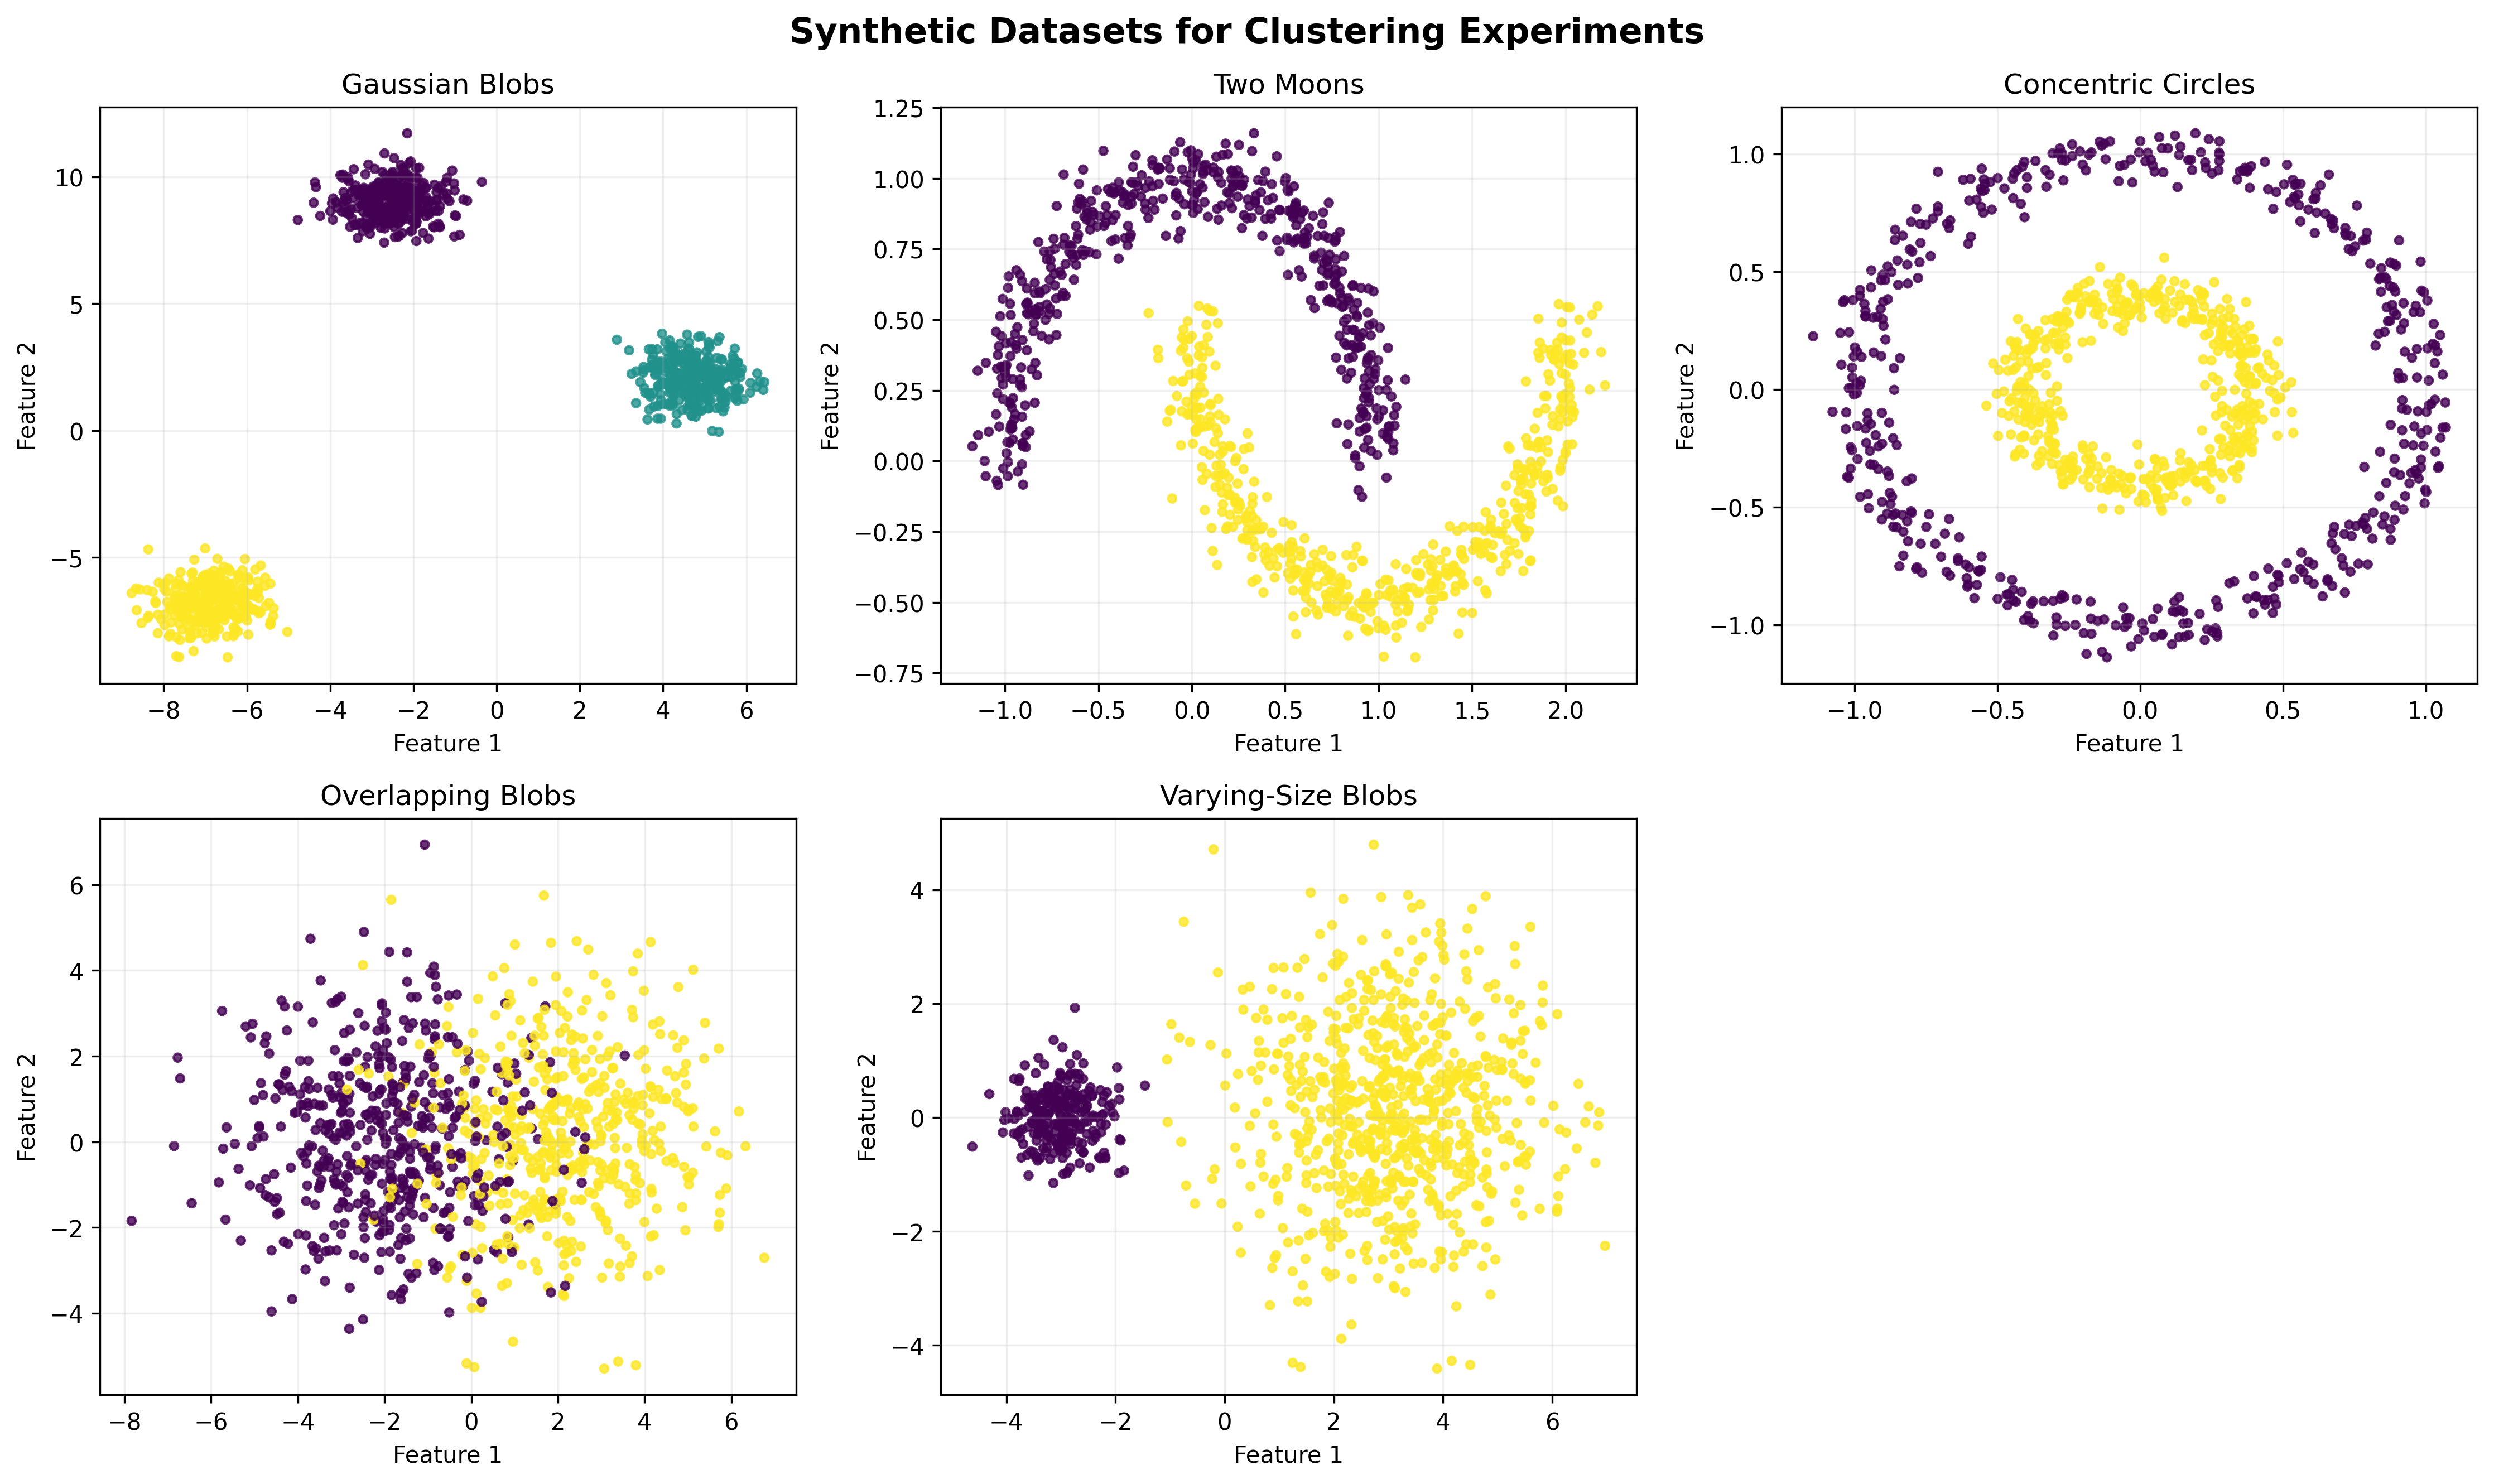
\includegraphics[width=0.9\textwidth]
    {../results/figures/dataset_overview.png}
    \caption{Overview of the five synthetic datasets used
    in the experiments.}
    \label{fig:datasets}
\end{figure}

\subsection{Evaluation Metrics}

We evaluate clustering performance using runtime,
Silhouette Score, and Adjusted Rand Index.

\subsubsection{Runtime}

Runtime measures the time required for an algorithm to fit
the dataset.

We measure the execution time of the clustering algorithm
using Python's \texttt{perf\_counter} function.

For the initial dataset comparison, we perform five executions
and report the average runtime.

For the dataset-size experiment, we perform five executions
and report the median runtime.

\subsubsection{Silhouette Score}

The Silhouette Score measures how similar a point is to its
own cluster compared with other clusters.

Its value ranges from $-1$ to $1$, where higher values generally
indicate better-separated clusters.

For larger datasets, we calculate the score using a reproducible
sample of up to 2,000 points to reduce evaluation time.

\subsubsection{Adjusted Rand Index}

The Adjusted Rand Index (ARI) measures the similarity between
the predicted cluster assignments and the known ground-truth
labels.

An ARI of 1 indicates perfect agreement, while a value near
0 indicates agreement comparable to random assignments.

Unlike the Silhouette Score, ARI uses the known labels and
therefore allows us to evaluate whether the algorithm recovered
the intended clusters.

% ==================================================
\section{Implementation}
% ==================================================

\subsection{Project Structure}

The project is implemented in Python and organized into
separate modules for dataset generation, clustering algorithms,
evaluation, and experimentation.

The main components include:

\begin{itemize}
    \item \texttt{generate\_data.py}: Generates the synthetic
    datasets used in the experiments.

    \item \texttt{kmeans.py}: Implements the K-Means
    clustering configuration.

    \item \texttt{hierarchical.py}: Implements Ward and
    Single linkage clustering.

    \item \texttt{evaluation.py}: Calculates runtime-related
    results, Silhouette Score, and ARI.

    \item \texttt{common.py}: Provides a shared experiment
    harness that executes an algorithm and returns its
    runtime and clustering quality metrics.

    \item \texttt{run\_experiments.py}: Runs the dataset
    characteristic and dataset-size experiments.

    \item \texttt{plot\_size\_results.py}: Generates
    visualizations of runtime and clustering quality
    as dataset size increases.
\end{itemize}

\subsection{Shared Experiment Harness}

To ensure consistent evaluation, we implemented a shared
\texttt{run\_experiment(dataset, algorithm)} function.

The function accepts a dataset containing the feature matrix
and ground-truth labels, along with an algorithm identifier.

It fits the selected clustering algorithm and returns:

\begin{itemize}
    \item Runtime in seconds
    \item Silhouette Score
    \item Adjusted Rand Index
\end{itemize}

The number of clusters is determined from the known
ground-truth labels. A fixed random seed is used for
reproducibility.

% ==================================================
\section{Experimental Results}
% ==================================================

\subsection{Comparison Across Dataset Characteristics}

We first evaluated all three algorithms on the five synthetic
datasets, each containing 1,000 samples.

Table~\ref{tab:initial-results} summarizes the preliminary
experimental results.

\begin{table}[H]
\centering
\caption{Initial clustering results across five datasets.}
\label{tab:initial-results}
\small
\begin{tabular}{llrr}
\toprule
\textbf{Dataset} & \textbf{Algorithm}
& \textbf{Silhouette} & \textbf{ARI} \\
\midrule

\multirow{3}{*}{Gaussian Blobs}
& K-Means & 0.8905 & 1.0000 \\
& Ward & 0.8905 & 1.0000 \\
& Single & 0.8905 & 1.0000 \\
\midrule

\multirow{3}{*}{Two Moons}
& K-Means & 0.4852 & 0.2433 \\
& Ward & 0.4837 & 0.2553 \\
& Single & 0.3300 & 1.0000 \\
\midrule

\multirow{3}{*}{Concentric Circles}
& K-Means & 0.3280 & -0.0010 \\
& Ward & 0.2643 & 0.0103 \\
& Single & 0.1552 & 1.0000 \\
\midrule

\multirow{3}{*}{Overlapping Blobs}
& K-Means & 0.4244 & 0.5987 \\
& Ward & 0.4017 & 0.5208 \\
& Single & 0.3593 & 0.0000 \\
\midrule

\multirow{3}{*}{Varying-Size Blobs}
& K-Means & 0.6345 & 0.9293 \\
& Ward & 0.6335 & 0.9915 \\
& Single & 0.2941 & -0.0013 \\

\bottomrule
\end{tabular}
\end{table}

\subsubsection{Preliminary Observations}

Several observations emerge from the initial experiments:

\begin{itemize}

    \item \textbf{Gaussian Blobs:}
    All three algorithms achieved perfect ARI scores,
    indicating that they successfully recovered the
    well-separated clusters.

    \item \textbf{Two Moons:}
    Single linkage achieved an ARI of 1.0, while
    K-Means and Ward produced substantially lower scores.
    This illustrates the advantage of Single linkage when
    identifying non-convex cluster shapes.

    \item \textbf{Concentric Circles:}
    Single linkage again achieved perfect ARI, whereas
    K-Means and Ward struggled to recover the nested
    cluster structure.

    \item \textbf{Overlapping Blobs:}
    K-Means achieved the highest ARI, followed by Ward.
    Single linkage performed poorly on this dataset.

    \item \textbf{Varying-Size Blobs:}
    Ward achieved the highest ARI, slightly outperforming
    K-Means. Single linkage did not recover the intended
    clusters successfully.

\end{itemize}

These results demonstrate that no single algorithm performs
best across every dataset characteristic.

\subsection{Effect of Dataset Size}

To investigate scalability, we generated Gaussian blob datasets
with increasing numbers of samples:

\[
n \in \{500, 1000, 2500, 5000, 10000, 20000\}
\]

Each algorithm was evaluated using five repeated executions,
with median runtime reported.

K-Means was evaluated at every dataset size. Due to the
memory requirements of hierarchical clustering, Ward and
Single linkage were evaluated only up to 5,000 samples.

\subsubsection{Runtime Results}

Table~\ref{tab:size-runtime} presents the measured median
runtime in seconds.

\begin{table}[H]
\centering
\caption{Median runtime by dataset size (seconds).}
\label{tab:size-runtime}
\begin{tabular}{rrrr}
\toprule
\textbf{Samples} & \textbf{K-Means}
& \textbf{Ward} & \textbf{Single} \\
\midrule
500    & 0.038910 & 0.008827 & 0.005023 \\
1,000  & 0.021430 & 0.032645 & 0.010787 \\
2,500  & 0.021738 & 0.251912 & 0.089808 \\
5,000  & 0.036179 & 0.928655 & 0.197543 \\
10,000 & 0.037967 & -- & -- \\
20,000 & 0.054852 & -- & -- \\
\bottomrule
\end{tabular}
\end{table}

\begin{figure}[H]
    \centering
    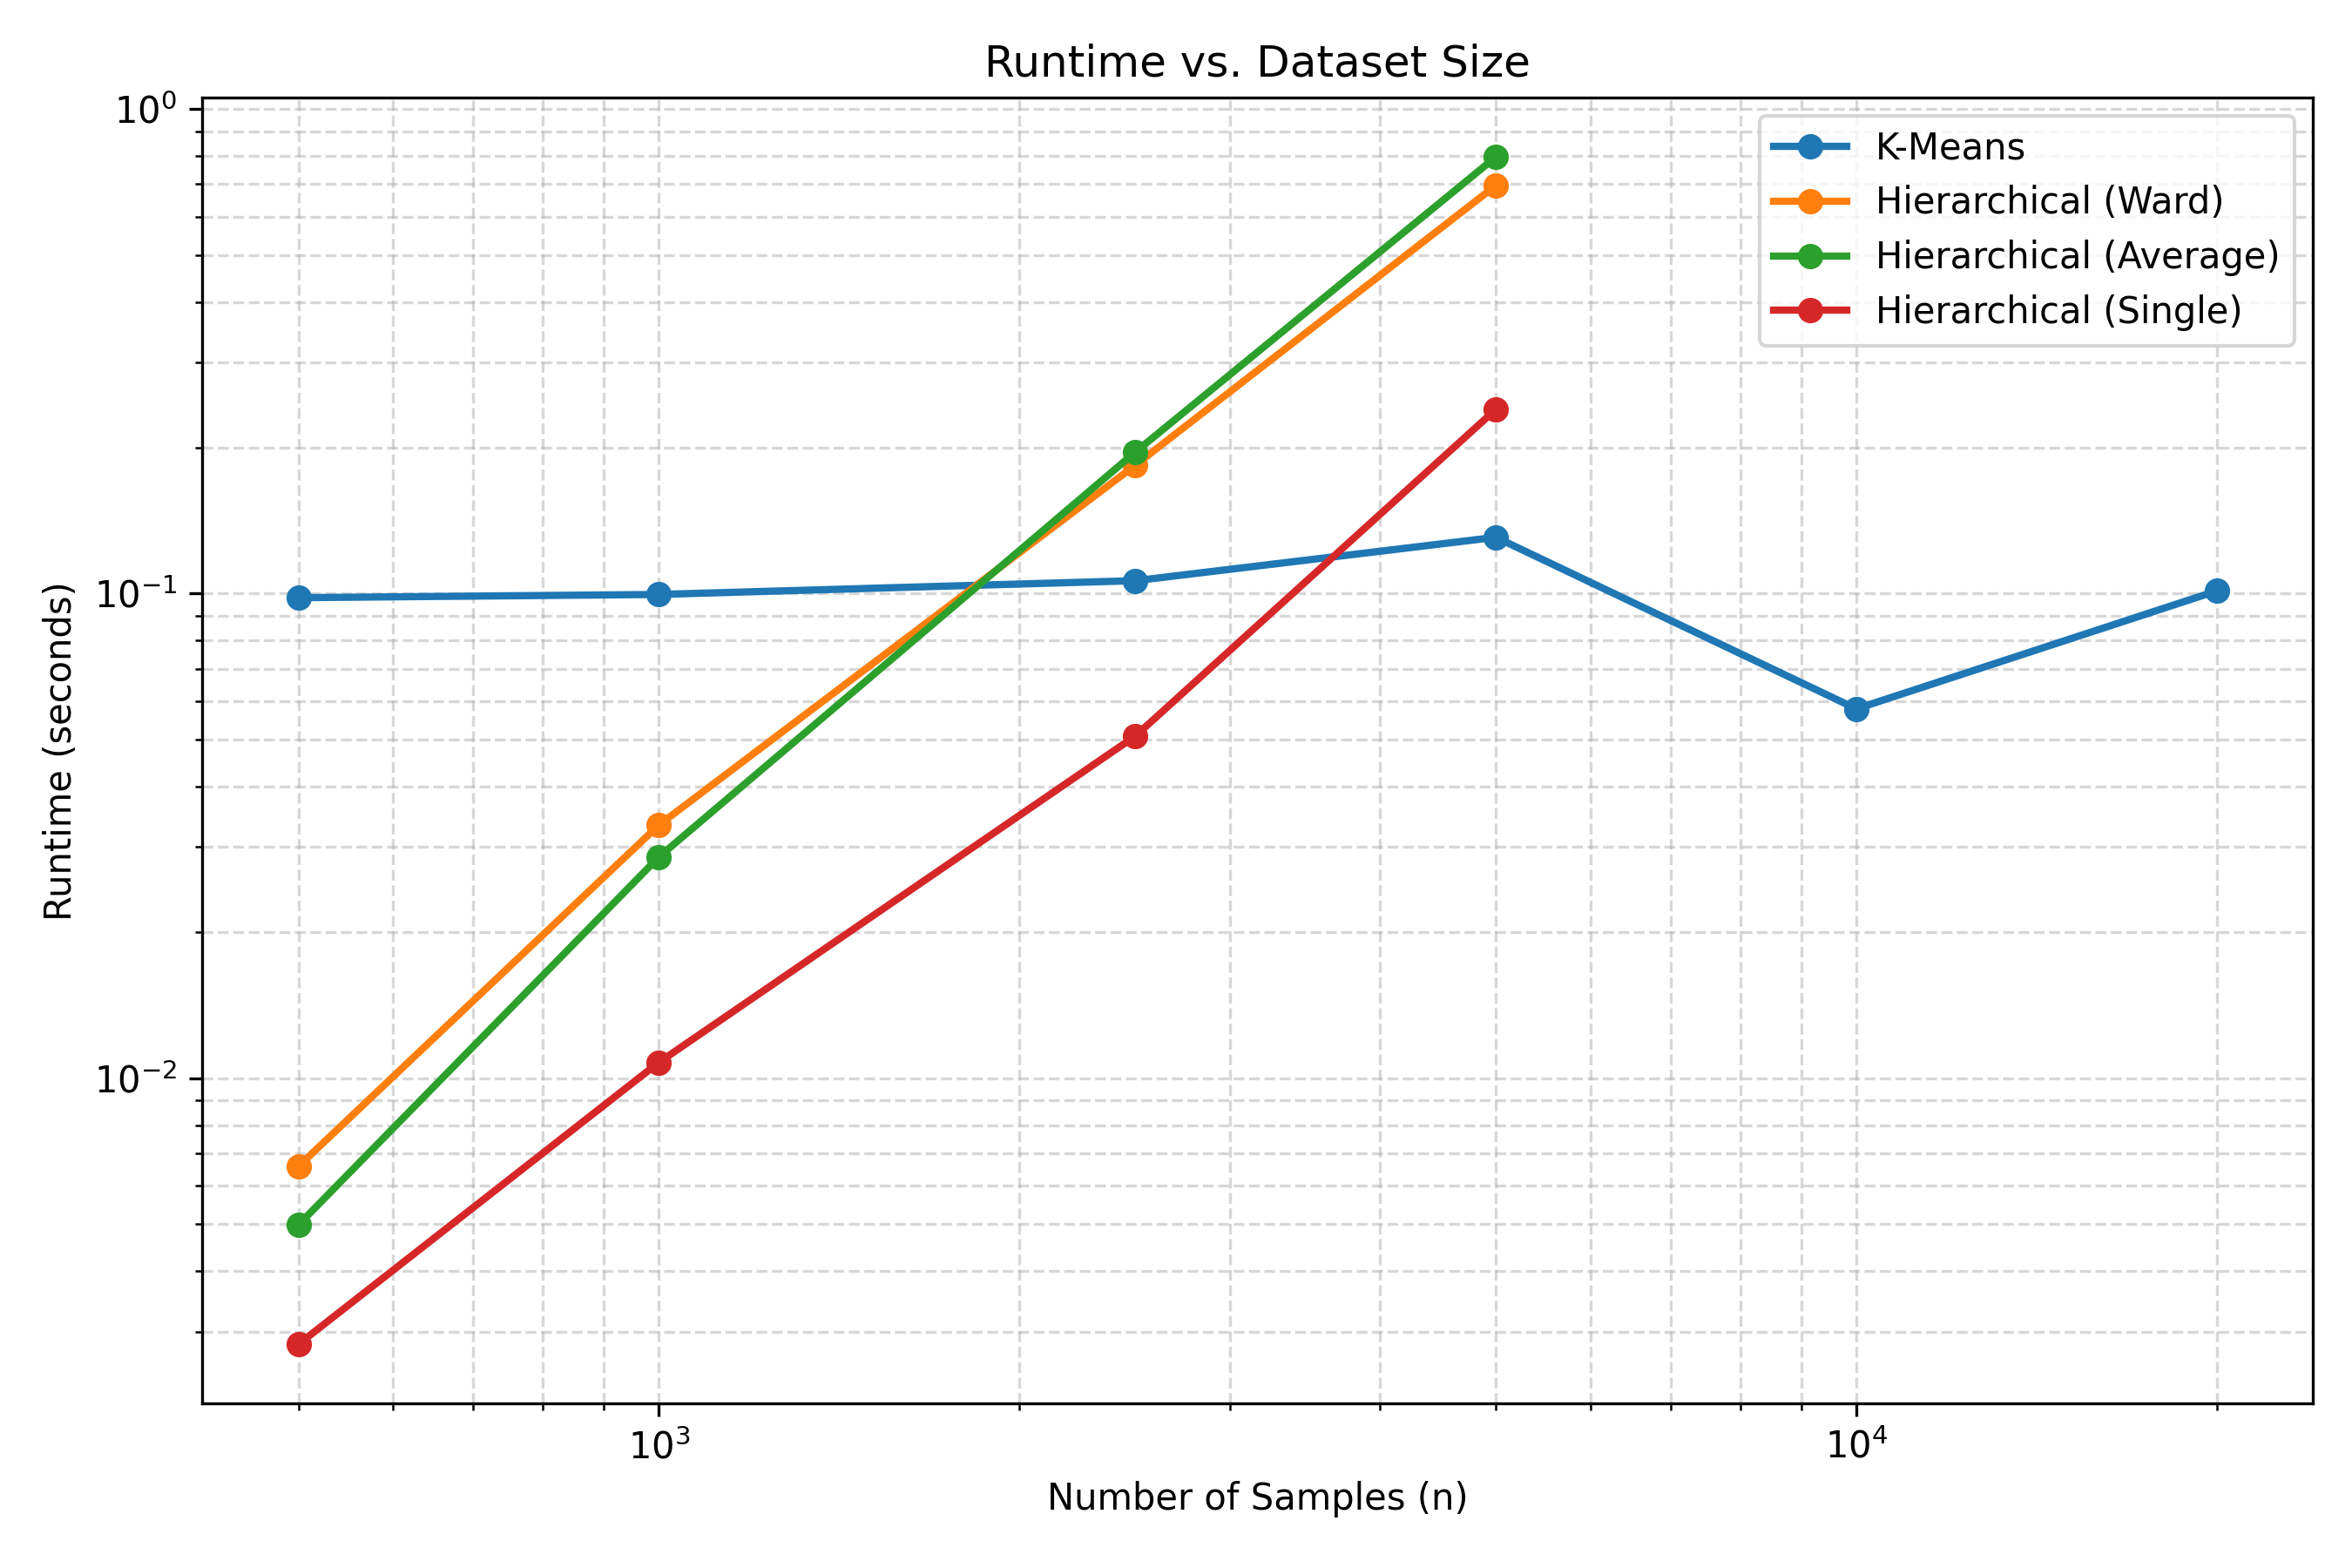
\includegraphics[width=0.95\textwidth]
    {../results/figures/runtime_vs_size.png}
    \caption{Runtime comparison as the number of samples
    increases. Both axes use logarithmic scales.}
    \label{fig:runtime}
\end{figure}

The results show that K-Means maintained relatively low
runtime as the dataset increased from 500 to 20,000 samples.

Ward linkage experienced a substantial increase in runtime,
reaching approximately 0.93 seconds at 5,000 samples.
Single linkage was faster than Ward at the tested sizes,
although its runtime also increased as the dataset grew.

These preliminary results suggest that K-Means is more
computationally scalable for this dataset.

\subsubsection{Clustering Quality Results}

Table~\ref{tab:size-quality} summarizes the clustering
quality metrics across dataset sizes.

\begin{table}[H]
\centering
\caption{Clustering quality by dataset size.}
\label{tab:size-quality}
\begin{tabular}{rrrrrr}
\toprule
\textbf{Samples}
& \multicolumn{3}{c}{\textbf{ARI}}
& \multicolumn{2}{c}{\textbf{Silhouette}} \\
\cmidrule(lr){2-4}
\cmidrule(lr){5-6}
& \textbf{K-Means}
& \textbf{Ward}
& \textbf{Single}
& \textbf{K-Means}
& \textbf{All} \\
\midrule
500    & 1.0000 & 1.0000 & 1.0000 & 0.8908 & 0.8908 \\
1,000  & 1.0000 & 1.0000 & 1.0000 & 0.8905 & 0.8905 \\
2,500  & 1.0000 & 1.0000 & 1.0000 & 0.8895 & 0.8895 \\
5,000  & 1.0000 & 1.0000 & 1.0000 & 0.8875 & 0.8875 \\
10,000 & 1.0000 & -- & -- & 0.8888 & 0.8888 \\
20,000 & 1.0000 & -- & -- & 0.8906 & 0.8906 \\
\bottomrule
\end{tabular}
\end{table}

\begin{figure}[H]
    \centering
    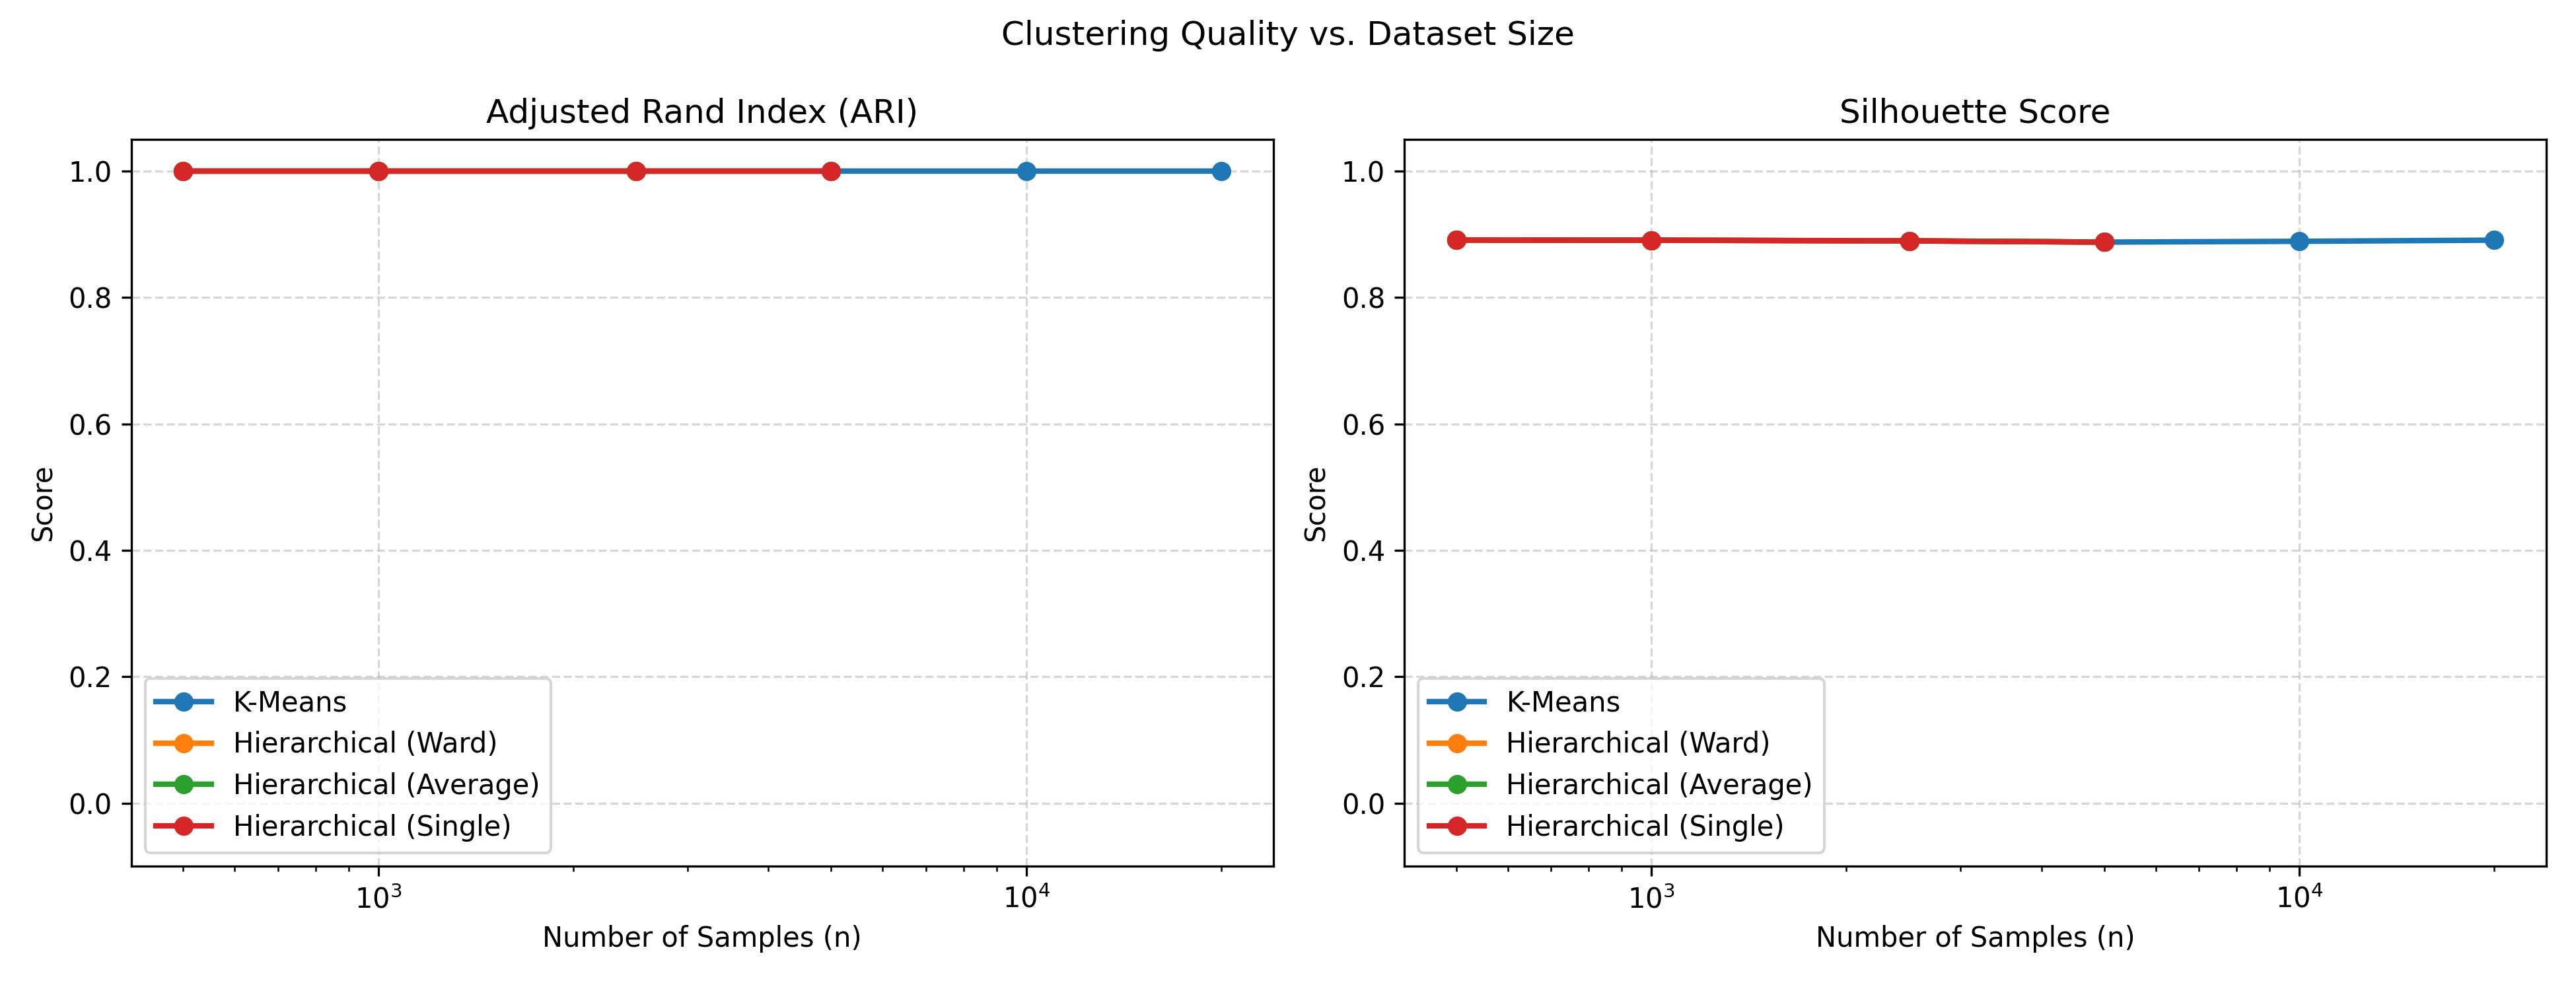
\includegraphics[width=\textwidth]
    {../results/figures/quality_vs_size.png}
    \caption{ARI and Silhouette Score as the number of
    samples increases. The hierarchical results overlap
    with the K-Means results at the tested sizes.}
    \label{fig:quality}
\end{figure}

All three algorithms achieved an ARI of 1.0 across the
tested sizes. Silhouette scores remained close to 0.89,
indicating that clustering quality remained stable as
the dataset increased.

This suggests that all three methods can successfully
identify the well-separated Gaussian clusters, even as
the number of samples increases.

% ==================================================
\section{Discussion}
% ==================================================

The preliminary experiments illustrate the importance of
considering both dataset structure and computational cost
when selecting a clustering algorithm.

K-Means performed well on compact, well-separated clusters
and maintained relatively low runtime as dataset size increased.

However, its centroid-based approach struggled with
non-convex structures such as Two Moons and Concentric
Circles.

Single linkage was particularly effective on these irregular
shapes, achieving perfect ARI on both datasets. However,
it performed poorly on the overlapping and varying-size
datasets.

Ward linkage generally produced compact clusters and
performed competitively with K-Means on Gaussian and
varying-size blobs.

An important observation is that Silhouette Score and ARI
do not always agree. For example, on Two Moons and
Concentric Circles, K-Means achieved higher Silhouette
Scores than Single linkage despite having substantially
lower ARI.

This demonstrates that a metric favoring compact,
well-separated clusters does not necessarily reward
recovery of the underlying non-convex structure.

\subsection{Limitations}

The current experiments have several limitations:

\begin{itemize}

    \item The datasets are synthetic and may not represent
    the complexity of real-world data.

    \item The dataset-size experiment uses Gaussian blobs,
    so its scalability findings should not automatically
    be generalized to other cluster structures.

    \item Hierarchical clustering was capped at 5,000
    samples due to memory considerations. Therefore,
    its runtime at larger dataset sizes was not measured.

    \item Silhouette Scores for datasets larger than
    2,000 samples are estimated using a reproducible
    sample rather than every data point.

    \item Runtime measurements can vary with hardware,
    system activity, and implementation details.

\end{itemize}

% ==================================================
\section{Conclusion}
% ==================================================

This project compares K-Means and two forms of
Agglomerative Hierarchical Clustering across different
synthetic dataset structures and sizes.

Our preliminary findings suggest that algorithm performance
depends heavily on the underlying data distribution.

K-Means is computationally efficient and performs well on
compact, well-separated clusters. Single linkage can recover
irregular cluster structures that K-Means struggles with,
while Ward linkage provides competitive results on several
compact and varying-size datasets.

The dataset-size experiment also suggests that K-Means
maintains better computational scalability than the
hierarchical approaches tested.

Overall, the experiments demonstrate that clustering
algorithm selection involves a trade-off between
computational efficiency and the ability to recover
different types of cluster structures.

% ==================================================
\section{Future Work}
% ==================================================

The following work can further strengthen the project:

\begin{itemize}

    \item Repeat runtime experiments with warm-up runs
    and additional repetitions.

    \item Investigate the effect of cluster separation
    and density more systematically.

    \item Explore larger datasets for hierarchical
    clustering where computational resources permit.

    \item Investigate additional clustering approaches
    for comparison, if the project scope allows.

    \item Incorporate feedback from the class presentation
    into the final report.

\end{itemize}

% ==================================================
\section{Group Contributions}
% ==================================================

The project is a collaborative effort. The following
section will be completed by the group before submission.

\begin{itemize}

    \item \textbf{Iaroslav Volkov:}
    [Describe contributions.]

    \item \textbf{Elizabeth Lam:}
    [Describe contributions.]

    \item \textbf{Fay Lee:}
    [Describe contributions.]

\end{itemize}

All group members contributed to the project through
[add details about collaboration, experimentation,
analysis, and report preparation].

% ==================================================
\section{Use of Generative AI}
% ==================================================

[Describe the use of generative AI tools in accordance
with the course requirements. Include the tools used,
their contributions, and how the group reviewed and
validated the resulting work.]

% ==================================================
\section{References}
% ==================================================

% Add sources for:
% - K-Means
% - Agglomerative Hierarchical Clustering
% - Ward linkage
% - Single linkage
% - Silhouette Score
% - Adjusted Rand Index
% - Scikit-learn implementation

\begin{thebibliography}{9}

\bibitem{placeholder}
[Add bibliographic references here.]

\end{thebibliography}

\end{document}
